\section{Preliminaries}\label{sec2}
In this section, we first introduce the basic concepts of differential privacy and differential privacy for time series. As for the latter, we mainly focus on different privacy levels of DP mechanisms used to analyze time series.

\subsection{Differential Privacy}
% differential privacy
Differential privacy is a rigorous and practical formalization that provides a quantitative measure of privacy leakage for an individual when participating in a database~\cite{Dwork2006}. In the nearly 20 years since its inception, differential privacy has become widely adopted as a privacy-preserving framework. Many companies, such as Microsoft~\cite{Ding2017}, Google~\cite{Erlingsson2014}, and Apple~\cite{Thakurta2017}, utilize differential privacy to collect users' data while providing privacy guarantees.  Additionally, the US Census Bureau adopted differential privacy for the 2020 decennial census~\cite{Dwork2019}.

Based on utilization scenarios, differential privacy can be broadly categorized into centralized differential privacy (CDP) and local differential privacy (LDP)~\cite{Yang2023}. Centralized differential privacy requires a trusted third party to act as the data curator, collecting data from users and releasing the processed results to the public. The trusted third party is assumed to safeguard private information and not disclose it. However, in many situations, such a trusted third party may not exist.  Consequently, local differential privacy has been proposed, allowing data to be sanitized locally before being uploaded. These two different  scenarios are depicted in Fig~\ref{cdp-ldp}, and their formal definitions are provided below.

\begin{figure}[htbp]
	\centering
		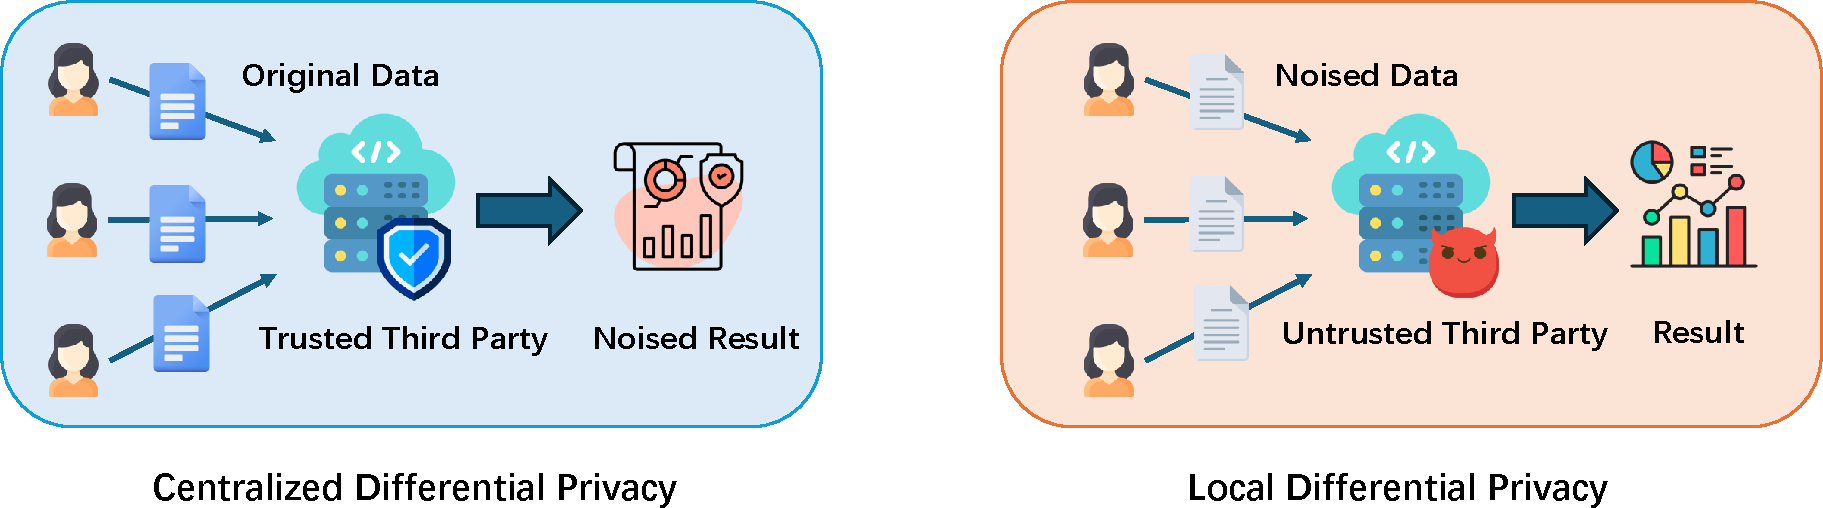
\includegraphics[width=0.7\textwidth]{submissions/submission4/figs/02-pre/cdp-ldp-crop.pdf}
	\caption{An illustration for centralized differential privacy and local differential privacy. In the context of centralized differential privacy, a trusted third party collects original data from users and adds noise to the processed result. In contrast, under  local differential privacy, users add noise to their data locally before uploading the noised data to the untrusted third party.}
	\label{cdp-ldp}
\end{figure}

\subsubsection{Centralized Differential Privacy (CDP)}
Before delving into the formal definition of centralized differential privacy, it is important to first elucidate some underlying concepts. We start with the definition of  neighboring datasets.
%Since CDP prevents distinguishing an individual from a group, datasets that differ by only one record from an individual are referred to as neighboring datasets~\cite{dwork2014algorithmic}.
\begin{definition}[Neighboring Datasets~\cite{dwork2014algorithmic, zhao2022survey, li2017differential}]
	Two datasets $D$ and $D'$ are \textit{neighboring} if they only differ by only one record. In \textit{Unbounded CDP}, $D$ can be obtained from $D'$ by adding or removing one record, whereas in \textit{Bounded DP}, $D$ can be obtained from $D'$ by replacing one record.
\end{definition}

\begin{definition}[$(\epsilon, \delta)$-Centralized Differential Privacy ($(\epsilon, \delta)$-CDP)~\cite{dwork2014algorithmic, zhao2022survey, li2017differential}] A randomized mechanism $\mathcal{M}$ satisfies $(\epsilon, \delta)$-centralized differential privacy if and only if for any two neighboring datasets $D$, $D'$, and any possible output $R\subseteq\mathrm{Range}(\mathcal{M})$, there is
	\begin{equation}
		\mathrm{Pr}[\mathcal{M}(D)=R]\le e^\epsilon\cdot \mathrm{Pr}[\mathcal{M}(D')=R]+\delta.\nonumber
	\end{equation}
When $\delta=0$, $\mathcal{M}$ satisfies $\epsilon$-centralized differential privacy.
\end{definition}



% local differentail privacy
\subsubsection{Local Differential Privacy (LDP)}
As we aforementioned, local differential privacy is adopted in a local mode. Compared with CDP, LDP requires more added noise to ensure privacy but does not need a trusted third party. Therefore, neighboring datasets in LDP can be any input from users.
\begin{definition}[$(\epsilon, \delta)$-local differential privacy ($(\epsilon, \delta)$-LDP)~\cite{zhao2022survey, li2017differential}]
A randomized mechanism $\mathcal{A}$ satisfies $(\epsilon, \delta)$-local differential privacy if and only if for any inputs $v$, $v'$, and any possible output $r\subseteq\mathrm{Range}(\mathcal{A})$, there is
\begin{equation}
	\mathrm{Pr}[\mathcal{A}(v)=r]\le e^\epsilon\cdot \mathrm{Pr}[\mathcal{A}(v')=r]+\delta.\nonumber
\end{equation}
When $\delta=0$, $\mathcal{A}$ satisfies $\epsilon$-local differential privacy which is also called pure-LDP~\cite{wang2017locally}.
\end{definition}

\subsubsection{Composition Theorems}
Under differential privacy (both CDP and LDP), there are two useful composition theorems~\cite{li2017differential}: sequential composition and parallel composition.

\begin{definition}[Sequential Composition~\cite{li2017differential}]
	Given a dataset $x$, and two mechanisms $M_1$, $M_2$ satisfy $(\epsilon_1, \delta_1)$-DP and $(\epsilon_2, \delta_2)$-DP, respectively, the mechanism $M=(M_1(x), M_2(x))$ satisfies $(\epsilon_1+\epsilon_2, \delta_1+\delta_2)$-DP.
\end{definition}

\begin{definition}[Parallel Composition~\cite{li2017differential}]
	Given a mechanism $M$ satisfy $(\epsilon, \delta)$-DP, and the $k$ disjoint separations of the dataset $x$ (i.e., $x_1\cup x_2\cup \cdots \cup x_k=x$), the release $M(x_1), M(x_2), \cdots, M(x_k)$ satisfies $(\epsilon, \delta)$-DP.
\end{definition}

% sequential composition


% parallel composition

\subsubsection{Pufferfish Privacy}
When providing privacy guarantees for correlated time series, differential privacy faces the challenge of excessive noise addition. Specifically, group differential privacy~\cite{dwork2014algorithmic} necessitates adding $O(T)$ noise for a  correlated time series with length $T$, leading to significant utility degradation. To address correlated data, pufferfish privacy, a generalized version of differential privacy, was proposed~\cite{kifer2014pufferfish}. In addition to the privacy budget $\epsilon$, pufferfish privacy requires three additional parameters~\cite{song2017pufferfish}: a set of secrets $\mathcal{S}$ representing users' private data, a set of secret pairs $\mathcal{Q}\subseteq \mathcal{S}\times \mathcal{S}$ that must remain indistinguishable, and a class of data distribution $\Theta$ indicating the correlation.
\begin{definition}[$\epsilon$-Pufferfish Privacy~\cite{song2017pufferfish}]
Give the parameters $\mathcal{S}$, $\mathcal{Q}$, and $\Theta$, a randomized mechanism $M$ satisfies $\epsilon$-pufferfish privacy if $\forall \theta\in \Theta $ with $X\sim \theta$, $\forall (s_i, s_j)\in \mathcal{Q}$, $\forall w\in \text{Range}(M)$, there is
\begin{equation}\nonumber
 \mathrm{Pr}(M(X)=w|s_i, \theta)\le e^\epsilon\cdot \mathrm{Pr}(M(X)=w|s_j, \theta),
\end{equation}
when $\mathrm{Pr[s_i|\theta]\ne 0}$ and $\mathrm{Pr[s_j|\theta]\ne 0}$.
\end{definition}
%For more detailed information about pufferfish privacy, readers are recommended to refer to~\cite{kifer2014pufferfish, song2017pufferfish}.





\subsubsection{Differential Privacy Mechanisms}
Given that noise addition from a distribution is a fundamental implementation of differential privacy, this technique is extensively used for statistical estimation. Numerous applications rely on count queries, including frequency estimation, histogram estimation, and top-$k$ item mining. Korolova et al. \cite{korolova2009releasing} introduced a mechanism for releasing search log histograms by adding Laplace noise. Xiao et al. \cite{xiao2010differential} proposed a wavelet-based mechanism to release range count queries. In the context of LDP, Wang et al. \cite{wang2017locally} reviewed existing mechanisms for frequency estimation and introduced two optimized approaches. Li et al. \cite{li2020estimating} developed a mechanism for estimating numerical data distributions. Wang et al. \cite{wang2019locallyhv} proposed a prefix extension mechanism to identify the top-$k$ frequent items within a large domain. Beyond count queries, many applications focus on sum or mean queries. Wang et al. \cite{wang2019collecting} devised a mechanism with optimized perturbation probability for numerical data under LDP. Xue et al. \cite{xue2022mean} introduced a mean estimation mechanism that supports personalized privacy budgets for each user. Zhou et al. \cite{zhou2022locally} developed a mechanism to estimate the mean of sparse vectors. To incorporate data knowledge, Wei et al. \cite{wei2024aaa} proposed an optimized mean estimation mechanism based on data distribution estimated in the initial phase under LDP. Beyond statistical estimations, data release for downstream tasks is another critical application. Ye et al. \cite{ye2020lf} proposed a mechanism to release edge information for clustering coefficient estimation. Ma et al. \cite{ma2024decision} developed a mechanism to construct decision trees under LDP, enhancing utility through the adoption of public data. Additionally, since the introduction of Differentially Private Stochastic Gradient Descent (DP-SGD) \cite{abadi2016deep}, numerous privacy-preserving learning-based mechanisms have been proposed under differential privacy.

Across the various scenarios, time series represent a unique research field due to their sequential nature and temporal dependencies. This adds complexity to ensuring differential privacy while maintaining data utility. In the following sections, we will introduce the concepts of time series under differential privacy.



\subsection{Differential Privacy for Time Series}
In this subsection, we will introduce the concept of time series and the specific definitions of differential privacy for time series, including various privacy levels. Additionally, we will provide a concise roadmap of this survey.

\subsubsection{Time Series}
In general, a time series is regarded an ordered sequence of values with finite length~\cite{esling2012time}, while data streams are continuously generated sequences with infinite length~\cite{silva2013data}. For ease of presentation, both are referred to as ``time series" in this paper, encompassing both finite and infinite settings.

% offline
%\begin{definition}[Finite Time Series~\cite{esling2012time, ruiz2021great}] A finite time series $S$ is an ordered sequences of values with a fixed length, i.e., $S=\{S_{t_1}, S_{t_2}, S_{t_3}, \cdots, S_{t_n}\}$. For simplicity, the timestamp is usually omitted, and a time series is denoted as $S=\{S_{1}, S_{2}, S_{3}, \cdots, S_{n}\}$. If any element $S_i\in \mathbb{R}$, the time series is called a univariate finite time series. Otherwise, if $S_i\in \mathbb{R}^d$,  it is referred to as a multivariate finite time series, meaning each element has $d$ dimensions.
%	
%\end{definition}


% online
\begin{definition}[Time Series~\cite{esling2012time, silva2013data, ruiz2021great}] A time series $S$ is an ordered sequences of values, i.e., $S=\{S_{t_1}, S_{t_2}, S_{t_3}, \cdots\}$. For simplicity, the timestamp is usually omitted, and a time series is denoted as $S=\{S_{1}, S_{2}, S_{3}, \cdots\}$. If any element $S_i\in \mathbb{R}$, the time series is called a univariate infinite time series. Otherwise, the time series is a multivariate infinite time series if $S_i\in \mathbb{R}^d$, namely, each element is with $d$ dimensions.
\end{definition}

Note that if a time series has a finite length, it is called a finite time series. Otherwise, it is referred to as an infinite time series.


\subsubsection{Privacy Levels}
In the context of time series, three major privacy levels have been proposed based on the privacy guarantees. Event-level privacy only protects a single element within a time series, $w$-event level privacy provides a privacy guarantee for a sequence of $w$ consecutive elements, and user-level privacy protects the entire time series. The corresponding definitions are provided below, with illustrations depicted in Fig.~\ref{privacy_level}.

\begin{definition}[Event-Level Adjacent Time Series~\cite{Kellaris14}]
	For two time series $S$ and $S'$, they are event-level adjacent if
	\begin{enumerate}
		\item [1)] There exists a timestamp $i$, $S_i\ne S'_i$;
		\item [2)] For any other timestamp $j$,  $S_j= S'_j.$
	\end{enumerate}
\end{definition}

\begin{definition}[Event-Level Privacy~\cite{Kellaris14}] A randomized mechanism $\mathcal{M}$ satisfies $(\epsilon, \delta)$-event-level differential privacy if and only if for any two event-level adjacent time series $S$, $S'$, and any possible output $R\subseteq\mathrm{Range}(\mathcal{M})$, there is
	\begin{equation}
		\mathrm{Pr}[\mathcal{M}(S)=R]\le e^\epsilon\cdot \mathrm{Pr}[\mathcal{M}(S')=R]+\delta.\nonumber
	\end{equation}
	When $\delta=0$, $\mathcal{M}$ satisfies $\epsilon$-event-level differential privacy.
\end{definition}

\begin{definition}[$w$-Event Level Adjacent Time Series~\cite{Kellaris14}]
	For two time series $S$ and $S'$, they are  $w$-event level adjacent if
	\begin{enumerate}
		\item [1)] There exists $w$ consecutive timestamp $\{k, k+1, \cdots, k+w-1\}$ and for any $i \in \{k, k+1, \cdots, k+w-1\}$, $S_i\ne S'_i$;
		\item [2)] For any other timestamp $j$,  $S_j= S'_j.$
	\end{enumerate}
\end{definition}

\begin{definition}[$w$-Event Level Privacy] A randomized mechanism $\mathcal{M}$ satisfies $(\epsilon, \delta)$-$w$-event level differential privacy if and only if for any two $w$-event level adjacent time series $S$, $S'$, and any possible output $R\subseteq\mathrm{Range}(\mathcal{M})$, there is
	\begin{equation}
		\mathrm{Pr}[\mathcal{M}(S)=R]\le e^\epsilon\cdot \mathrm{Pr}[\mathcal{M}(S')=R]+\delta.\nonumber
	\end{equation}
	When $\delta=0$, $\mathcal{M}$ satisfies $\epsilon$-$w$-event level differential privacy.
\end{definition}

\begin{definition}[User-Level Adjacent Time Series]
	For two time series $S$ and $S'$, they are user-level adjacent if for all timestamps $t_{u_i}=\{t_1, t_2, \cdots , t_k\}$  from any user $u_i$, there is $S_j\ne S'_j, \forall j\in t_{u_i}$. Note that $t_{u_i}$ can be infinite for infinite time series.
\end{definition}

\begin{definition}[User-Level Privacy] A randomized mechanism $\mathcal{M}$ satisfies $(\epsilon, \delta)$-user-level differential privacy if and only if for any two user-level adjacent time series $S$, $S'$, and any possible output $R\subseteq\mathrm{Range}(\mathcal{M})$, there is
	\begin{equation}
		\mathrm{Pr}[\mathcal{M}(S)=R]\le e^\epsilon\cdot \mathrm{Pr}[\mathcal{M}(S')=R]+\delta.\nonumber
	\end{equation}
	When $\delta=0$, $\mathcal{M}$ satisfies $\epsilon$-user-level differential privacy.
\end{definition}

\begin{figure}[H]
	\centering
	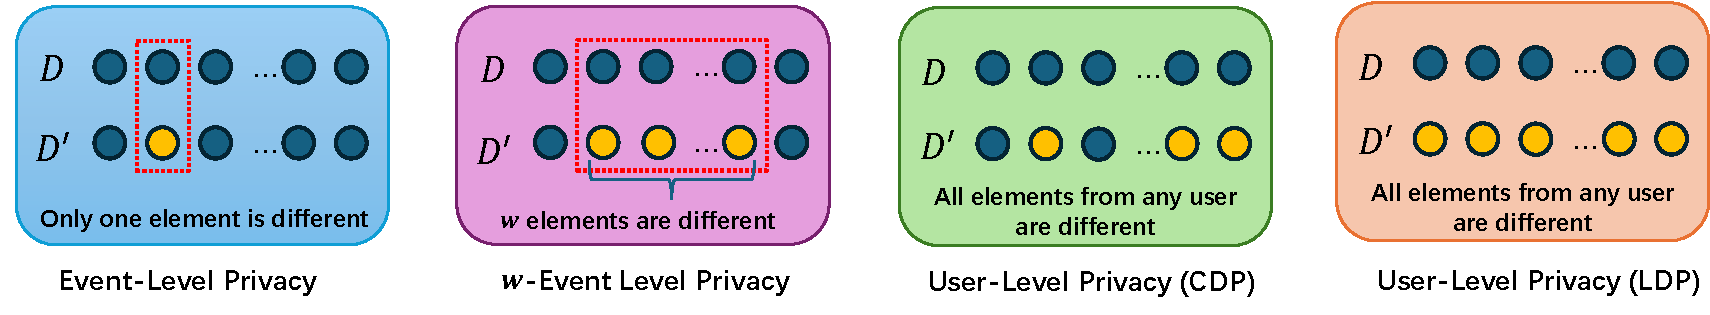
\includegraphics[width=0.8\textwidth]{submissions/submission4/figs/02-pre/privacy_level-crop.pdf}
	\caption{An illustration for privacy levels. In terms of event-level privacy, there is only one element different in the neighboring datasets. While for the $w$-event level privacy, there are $w$ consecutive elements that differ in the neighboring datasets. For user-level privacy, all the elements from any user can be different in the neighboring datasets. Note that under LDP, the two user-level adjacent time series are from different users, which means the elements could be entirely different. }
	\label{privacy_level}
\end{figure}


Obviously, event-level privacy provides the lowest level of privacy but requires the least amount of noise. Conversely, user-level privacy guarantees the strongest privacy but necessitates the largest amount of noise, which can significantly degrade utility.


\subsection{Roadmap of This Survey}
Since count queries and sum/mean queries are fundamental statistical operations, many advanced queries and downstream applications are derived from them. This survey begins with a review on count queries, followed by a discussion of sum/mean queries.  Each subsection on these queries starts with an introduction to the concepts, followed by a review of their downstream applications. Subsequently, we introduce data release mechanisms designed to publicize data for downstream tasks. Given the popularity of location based services in time series applications, we dedicate a separate section to trajectories, reviewing the literature on  location perturbation, temporal correlation issues, and trajectory release. To suggest future directions, we propose open challenges related to privacy models, temporal correlation-based attacks, complex data types, and learning-based problems. The roadmap for this survey is illustrated in Fig.~\ref{rm}.
\begin{figure}[htbp]
	\makebox[\textwidth][c]{%
	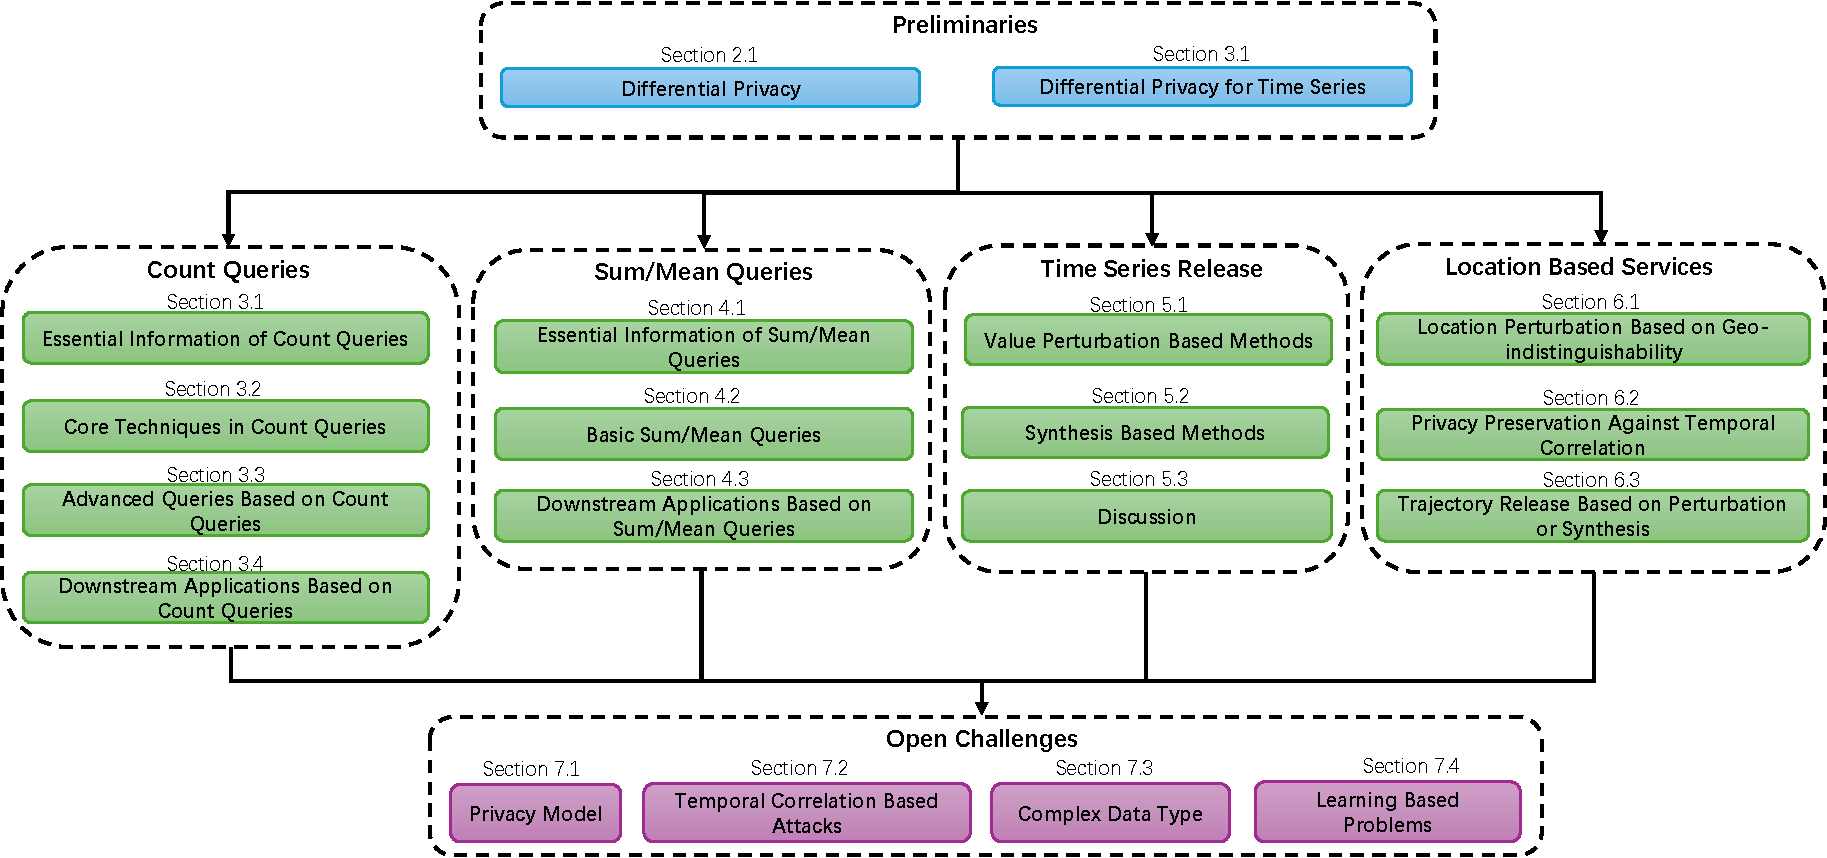
\includegraphics[width=1.1\textwidth]{submissions/submission4/figs/02-pre/roadmap-crop.pdf}
}
	\caption{Roadmap of this survey.}
	\label{rm}
\end{figure}








